\subsection{Parameters identification}
\label{subsec:parameters_identification}

In order to control the system, we need to identify its parameters.

To do so, different tests type will be performed, such as:

\begin{enumerate}
    \item Direct measurement: measure all the quantity of the system that can be directly measured or retrieved from well established literature;
    \item Sensors characterization: create the mapping between the position of the ball and the output voltage of the infrared sensor and study the variance of all the sensors used internally in the control unit;
    \item Control to voltage: observe the relation between the control signal and the effective voltage applied to the coils;
    \item Inductances characterization: identify all the parameters needed to characterize inductances, based on the model proposed in Equation \ref{eq:model_for_inductance};
    \item Force validation: measure the force applied to the ball by the inductance in order to validate both the model and the parameters identified in the previous tests.
\end{enumerate}

Except for the first test, all the others will be performed leveraging the data acquisition system included in the \texttt{Inteco} control unit.

\subsubsection{Direct measurement}
\label{subsubsec:direct_measurement}

In this section, we will measure all the quantities that can be directly measured or retrieved from well established literature.

Most of the following parameters can be directly measured using a scale and a caliper, respectively.
By doing so, we will have the following values:

\begin{table}[H]

    \centering
    \begin{tabular}{|c|c|c|}
        \hline
        \textbf{Parameter} & \textbf{Value} & \textbf{Units} \\
        \hline
        $g$                & $9.81$         & $m/s^2$        \\
        $m$                & $0.06157$      & $kg$           \\
        $r$                & $0.06125/2$    & $m$            \\
        $H$                & $0.098$        & $m$            \\
        \hline
    \end{tabular}

    \caption{Directly measured parameters and constants}
    \label{tab:directly_measured_parameters}

\end{table}

Also from literature, and in particular from the datasheet of the \texttt{Inteco} control unit, we can retrieve the following values about the literature model proposed in Equation \ref{eq:simplified_equations_of_motion_final}:

\begin{table}[H]

    \centering
    \begin{tabular}{|c|c|c|}
        \hline
        \textbf{Parameter} & \textbf{Value}         & \textbf{Units} \\
        \hline
        $F_{emP1}$         & $1.7521 \cdot 10^{-2}$ & $H$            \\
        $F_{emP2}$         & $5.8231 \cdot 10^{-3}$ & $m$            \\
        $f_{iP1}$          & $1.4142 \cdot 10^{-4}$ & $m \cdot s$    \\
        $f_{iP2}$          & $4.5626 \cdot 10^{-3}$ & $m$            \\
        $c_i$              & $0.0243$               & $A$            \\
        $k_i$              & $2.5165$               & $A$            \\
        \hline
    \end{tabular}

    \caption{Literature parameters}
    \label{tab:literature_parameters}

\end{table}


\subsubsection{Sensors characterization}
\label{subsubsec:sensors_characterization}

\hl{To be rewritten in a better form.}

We need to create the mapping between the position of the ball and the output voltage of the infrared sensor.
To do so, we simply create an array of points where we measure the position of the ball using a caliper and the output voltage of the infrared sensor using the data acquisition system included in the \texttt{Inteco} control unit.

The obtained data is shown in Figure \ref{fig:position_to_voltage}.

\begin{figure}[H]
    \centering
    % \includegraphics[width=0.6\textwidth]{img/MATLAB/identification/position_to_voltage.pdf}
    \caption{Position to voltage identification}
    \label{fig:position_to_voltage}
\end{figure}

As we can see, the relation between the position of the ball and the output voltage of the infrared sensor can be approximated as linear outside the limits of the sensor.

From the data obtained, one can clearly see that for distances of the ball from the upper coil grater than $\approx 20 [mm]$, the sensor reaches its saturation limit and the output voltage is constant.
Based on this observation, we can also impose that during simulations, the maximum distance of the ball from the upper coil is $20 [mm]$.

As a second step, we also need to study the variance of all the sensors used internally in the control unit.
We now suppose for both the infrared sensor for position and the current sensor that their model is Gaussian.
Based on this assumption, one can compute



\subsubsection{Control to voltage}
\label{subsubsec:control_to_voltage}

As said in the previous section of mathematical modeling, we need to identify the relation between the control signal and the effective voltage applied to the coils.
The control unit provided by \texttt{Inteco} it's programmed to receive a PWM duty cycle as input and to convert it into a voltage that is applied to the coils.
In order to identify this relation, we simply apply many duty cycles to the control unit and measure the corresponding voltage applied to the coils using a multimeter.

The output of this test is a series of points that can be fitted to a linear model having an initial black zone where the control action is not effective on the voltage applied to the coils.
In Figure \ref{fig:control_to_voltage} we can observe both the measured points, the linear fitting and the effective voltage applied considering the black zone.

\begin{figure}[H]
    \centering
    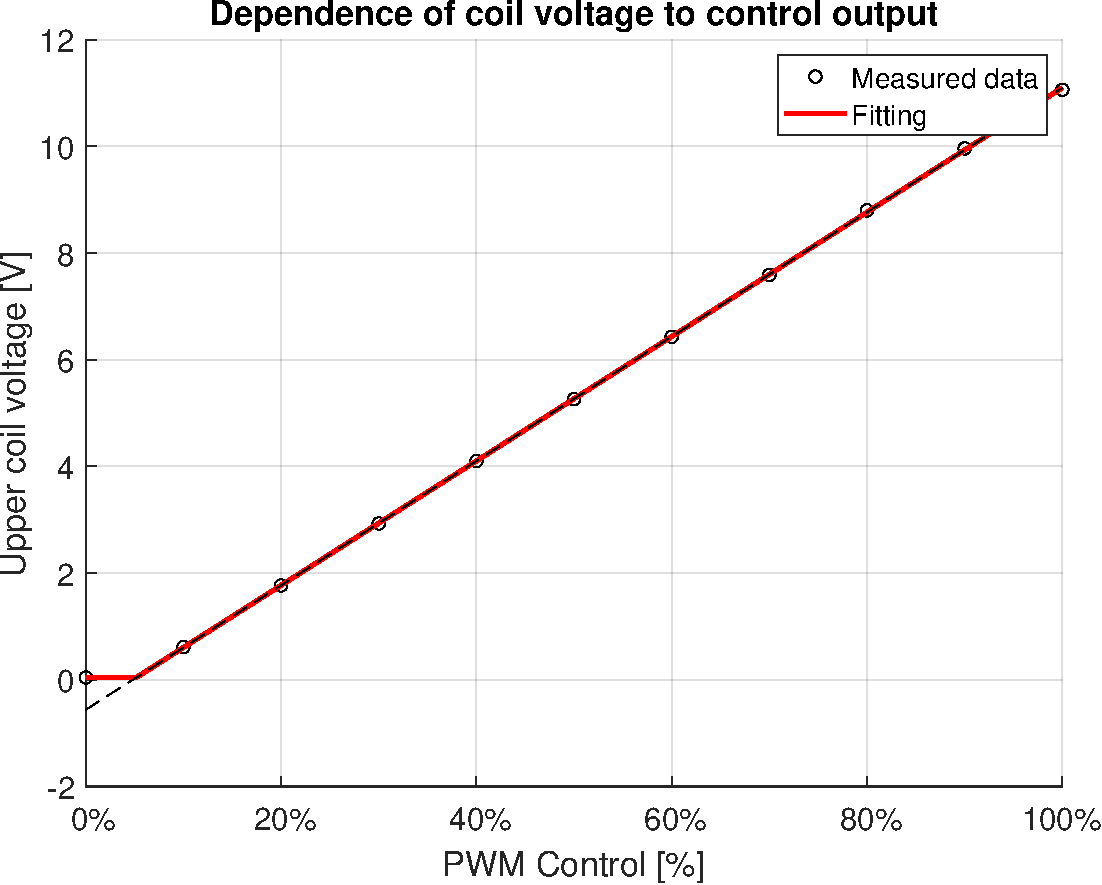
\includegraphics[width=0.6\textwidth]{img/MATLAB/identification/control_to_voltage.pdf}
    \caption{Control to voltage identification}
    \label{fig:control_to_voltage}
\end{figure}

As we can see, the linear model for the relation $V_* = f(U) = f(\text{PWM})$ is a good approximation outside the initial black zone control.
Because of this, we can consider the following control to voltage relation:

\begin{equation}
    V_* = \begin{cases}
        V_{*min}    & \text{if } U < U_{min}    \\
        k_* U + c_* & \text{if } U \geq U_{min}
    \end{cases}
\end{equation}

Where $V_{*min}$ is the minimum voltage applied to the coils when the control signal is zero, $u_{min}$ is the minimum control signal that is effective on the voltage applied to the coils, $k_*$ is the slope of the linear model and $c_*$ is the offset of the linear model.

The values of the parameters are shown in Table \ref{tab:control_to_voltage_parameters}.

\begin{table}[H]

    \centering
    \begin{tabular}{|c|c|c|}
        \hline
        \textbf{Parameter} & \textbf{Value}            & \textbf{Units} \\
        \hline
        $V_{*min}$         & $4.300000 \cdot 10^{-2}$  & $V$            \\
        $U_{min}$          & $5.179276$                & $\%$           \\
        $k_*$              & $1.165800 \cdot 10^{1}$   & $V/\%$         \\
        $c_*$              & $-5.608000 \cdot 10^{-1}$ & $V$            \\
        \hline
    \end{tabular}

    \caption{Control to voltage identification parameters}
    \label{tab:control_to_voltage_parameters}

\end{table}


\subsubsection{Inductances characterization}
\label{subsubsec:inductances_characterization}

A key parameter of the system is the inductance of the coils.

As already proposed in Equation \ref{eq:model_for_inductance}, the inductance of the coils cannot be considered constant and both its dependence on the current and the position of the ball must be taken into account when dealing with the magnetic levitation system.

In order to identify the inductance of the coils and all the parameters needed to characterize them, we have to measure the values of $L_1$ and $L_2$ for many currents and ball positions.
Once we have these values, we can fit the data to the model proposed in Equation \ref{eq:model_for_inductance} and identify the parameters.

Given a certain (fix in time) position of the ball and a certain current step input, we can measure the value of the inductance of the coils, knowing that:

\begin{equation}
    V = R I + \frac{d (L I)}{d t} = R I + \left( \frac{\partial L}{\partial I} I + L \right) \dot{I}
\end{equation}

If we suppose for a moment that the variation of the inductance with the current is negligible, we can obtain a closed form solution for the current in the RL circuit as follows:

\begin{equation}
    I(t) = \frac{V_{max}}{R_0} \left( 1 - e^{- \frac{R_0}{L_0} t} \right)
    \label{eq:current_in_rl_circuit}
\end{equation}

Given the previous equation, we can adopt the following strategy to fully characterize the inductance of the coils over the range of possible ball positions and currents:

\begin{enumerate}
    \item Fix the ball at a certain height ($z^*$);
    \item Apply a certain current step input to the system ($I^*$);
    \item Measure the current in the coils ($I(t)$);
    \item Fit the measured current to the model proposed in Equation \ref{eq:current_in_rl_circuit} and identify $L(z^*, I^*)$;
    \item Repeat from step 2 for different step inputs of currents;
    \item Repeat from step 1 for different ball positions.
\end{enumerate}

In Figure \ref{fig:inductance_characterization_currents} we can see on the left all the dynamics of the current in the coils for different step inputs of currents and different ball positions, while on the right we can see the fitting of the data to the model proposed in Equation \ref{eq:current_in_rl_circuit}.

\begin{figure}[H]
    \centering
    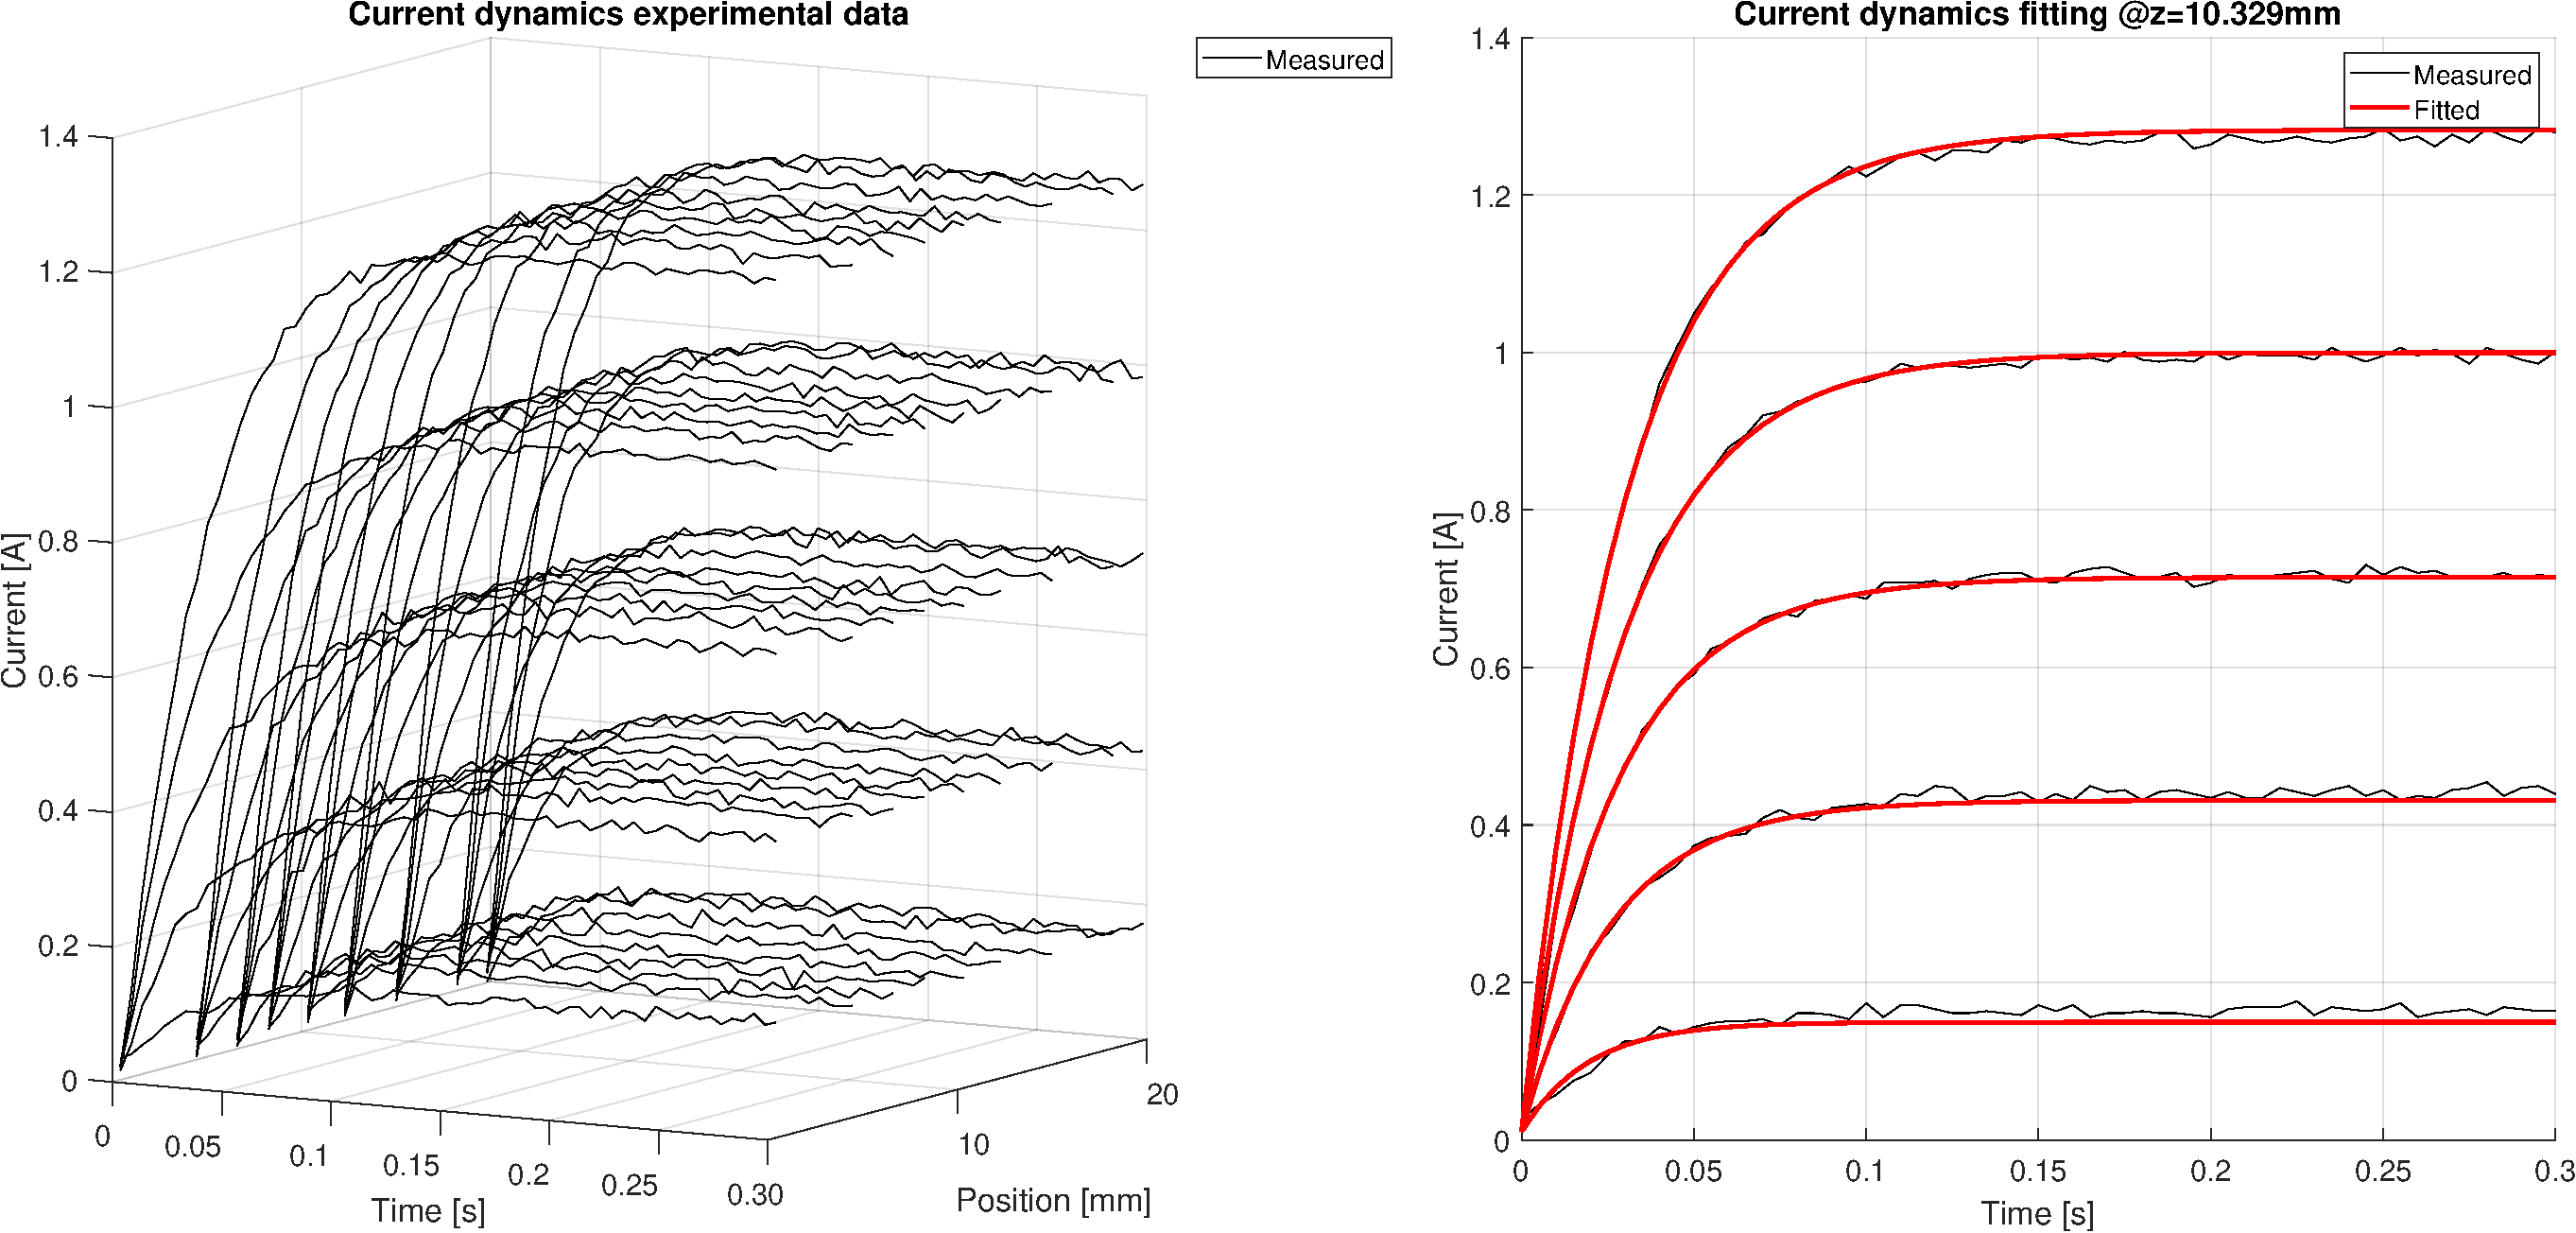
\includegraphics[width=1\textwidth]{img/MATLAB/identification/currents.pdf}
    \caption{Inductance characterization for different currents and ball positions}
    \label{fig:inductance_characterization_currents}
\end{figure}

From the right side of Figure \ref{fig:inductance_characterization_currents} we can see that the fitting of the data to the model proposed in Equation \ref{eq:current_in_rl_circuit} is optimal for middle values of the current, while it tends to underestimate and overestimate the current for low and high values of the current, respectively.
This behavior is probably due to the fact that the variation of the inductance with the current that has been neglected in the model of the current (Equation \ref{eq:current_in_rl_circuit}) is not negligible and should have been taken into account.

Thanks to the data obtained from the multiple tests, we can now fit the values of the inductance of the coils to the model proposed in Equation \ref{eq:model_for_inductance} and identify the parameters.
The obtained model fitting is shown in Figure \ref{fig:inductance_characterization_inductance}.

\begin{figure}[H]
    \centering
    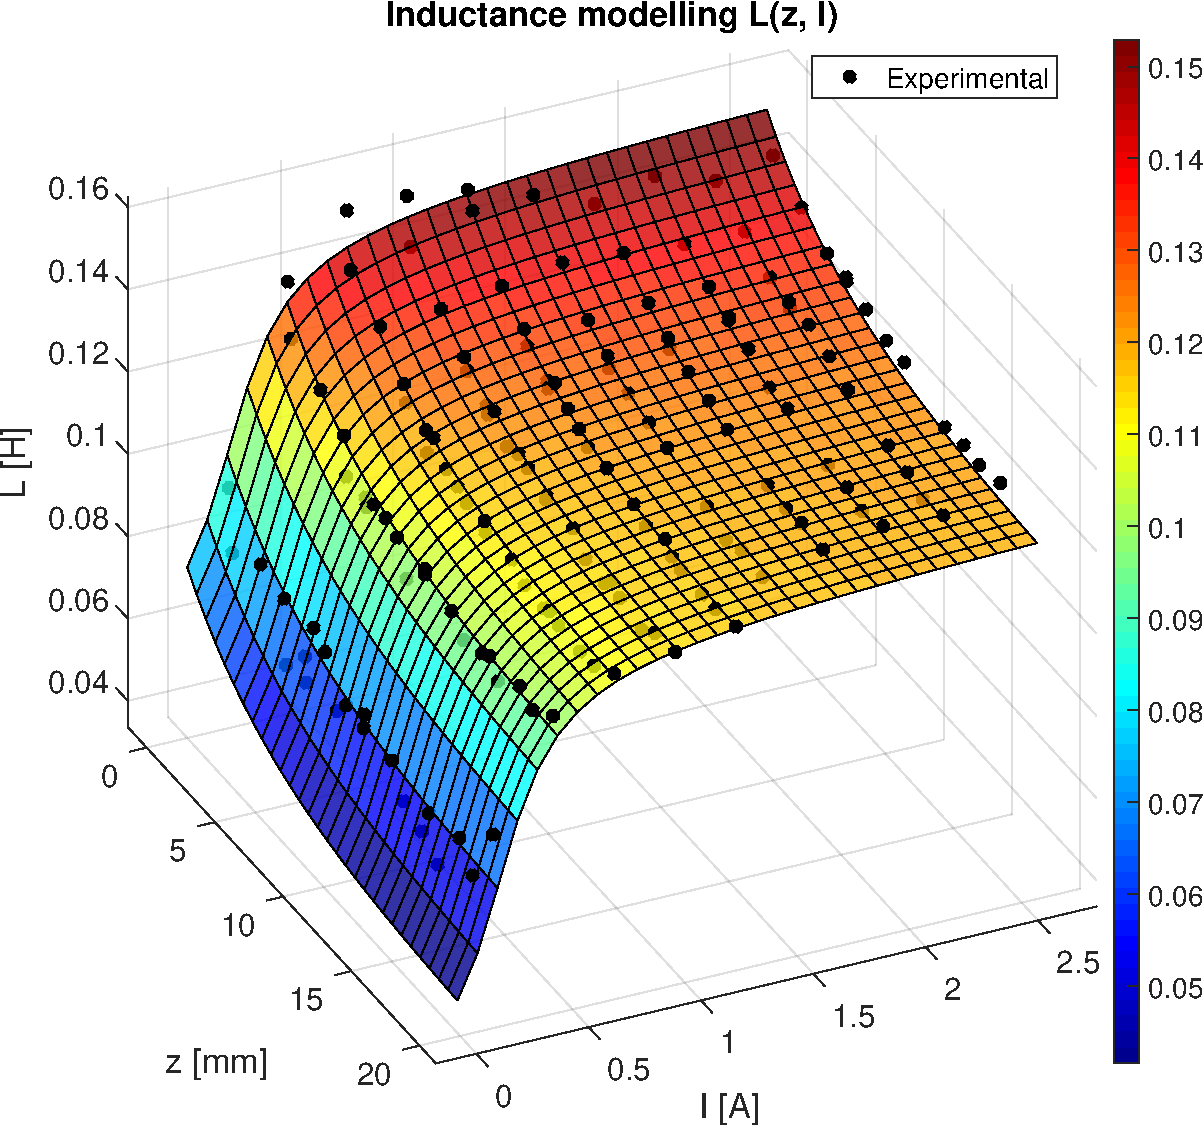
\includegraphics[width=0.6\textwidth]{img/MATLAB/identification/inductance.pdf}
    \caption{Inductance characterization}
    \label{fig:inductance_characterization_inductance}
\end{figure}

One can clearly see the $90$ points that have been used to fit the model proposed in Equation \ref{eq:model_for_inductance} and the obtained fitting.
The values of the parameters are shown in Table \ref{tab:inductance_characterization_parameters}.

\begin{table}[H]
    \centering
    \begin{tabular}{|c|c|c|}
        \hline
        \textbf{Parameter} & \textbf{Value}  & \textbf{Units} \\
        \hline
        $L_0$              & $4.106763e-02$  & $H$            \\
        $a_z$              & $2.155909e+02$  & $1/m$          \\
        $L_z$              & $4.288065e-02$  & $H$            \\
        $a_I$              & $2.553122e+00$  & $1/A$          \\
        $L_I$              & $-7.675453e-02$ & $H$            \\
        \hline
    \end{tabular}

    \caption{Inductance characterization parameters}
    \label{tab:inductance_characterization_parameters}

\end{table}

\subsubsection{Force validation}
\label{subsubsec:force_validation}

The last test that we will perform is the force validation.

Thanks to the data obtained from the previous tests, we should already be able to predict the force applied to the ball by the inductance.
In particular, we already know that the electromagnetic force applied to the ball is given by the following equation:

\begin{equation}
    F_{em} = \frac{1}{2} \frac{\partial L}{\partial z} I^2
\end{equation}

Because of the previously identified parameters, we have an analytical expression for the sensitivity of the inductance with respect to the position of the ball.
However, due to uncertainties in the identification of the parameters, we can expect some discrepancies between the predicted force and the measured one.

In order to quantify these discrepancies and validate the model, we will use a direct method to measure the force applied to the ball by the inductance and compare it with the predicted one.
To do so, we recall Equation \ref{eq:reduced_equations_of_motion_final} and in particular the equation relative to $\dot{v}$:

\begin{equation}
    \dot{v} = m^{-1} \left(\frac{1}{2} \frac{\partial L_1}{\partial z} I_1^2 + \frac{1}{2} \frac{\partial L_2}{\partial z} I_2^2 + m g  \right)
\end{equation}

If we consider the system at rest, we can simplify the equation as follows:

\begin{equation}
    0 = \frac{1}{2} \frac{\partial L_1}{\partial z} I_1^2 + \frac{1}{2} \frac{\partial L_2}{\partial z} I_2^2 + m g
\end{equation}

Supposing now that only the first coil is energized, we can further simplify the equation as follows:

\begin{equation}
    0 = \frac{1}{2} \frac{\partial L_1}{\partial z} I_1^2 + m g
\end{equation}

Which leads to:

\begin{equation}
    \frac{\partial L_1}{\partial z} = -2 \frac{m g}{I_1^2}
    \label{eq:sensitivity_of_inductance}
\end{equation}

This last equation basically tells us that in steady state conditions, when the ball is levitating (i.e. $\dot{z} = 0$ and not supported by any platform), the sensitivity of the inductance of the first coil has an analytical expression that can be directly measured by measuring the current in the first coil.

In order to follow this approach, a linearly increasing voltage has been applied to the first coil and the current corresponding to the levitation of the ball has been measured.
The test has been repeated for different initial positions of the ball, in order to fully characterize the dynamic inductance characteristics over the range of possible ball positions.

In Figure \ref{fig:levitation_current} we can see both the position of the ball and the current circulating in the first coil.
By identifying the current at which the ball starts to levitate (i.e. the ball starts to move upwards), we can than use Equation \ref{eq:sensitivity_of_inductance} to identify the dynamic inductance characteristics.

\begin{figure}[H]
    \centering
    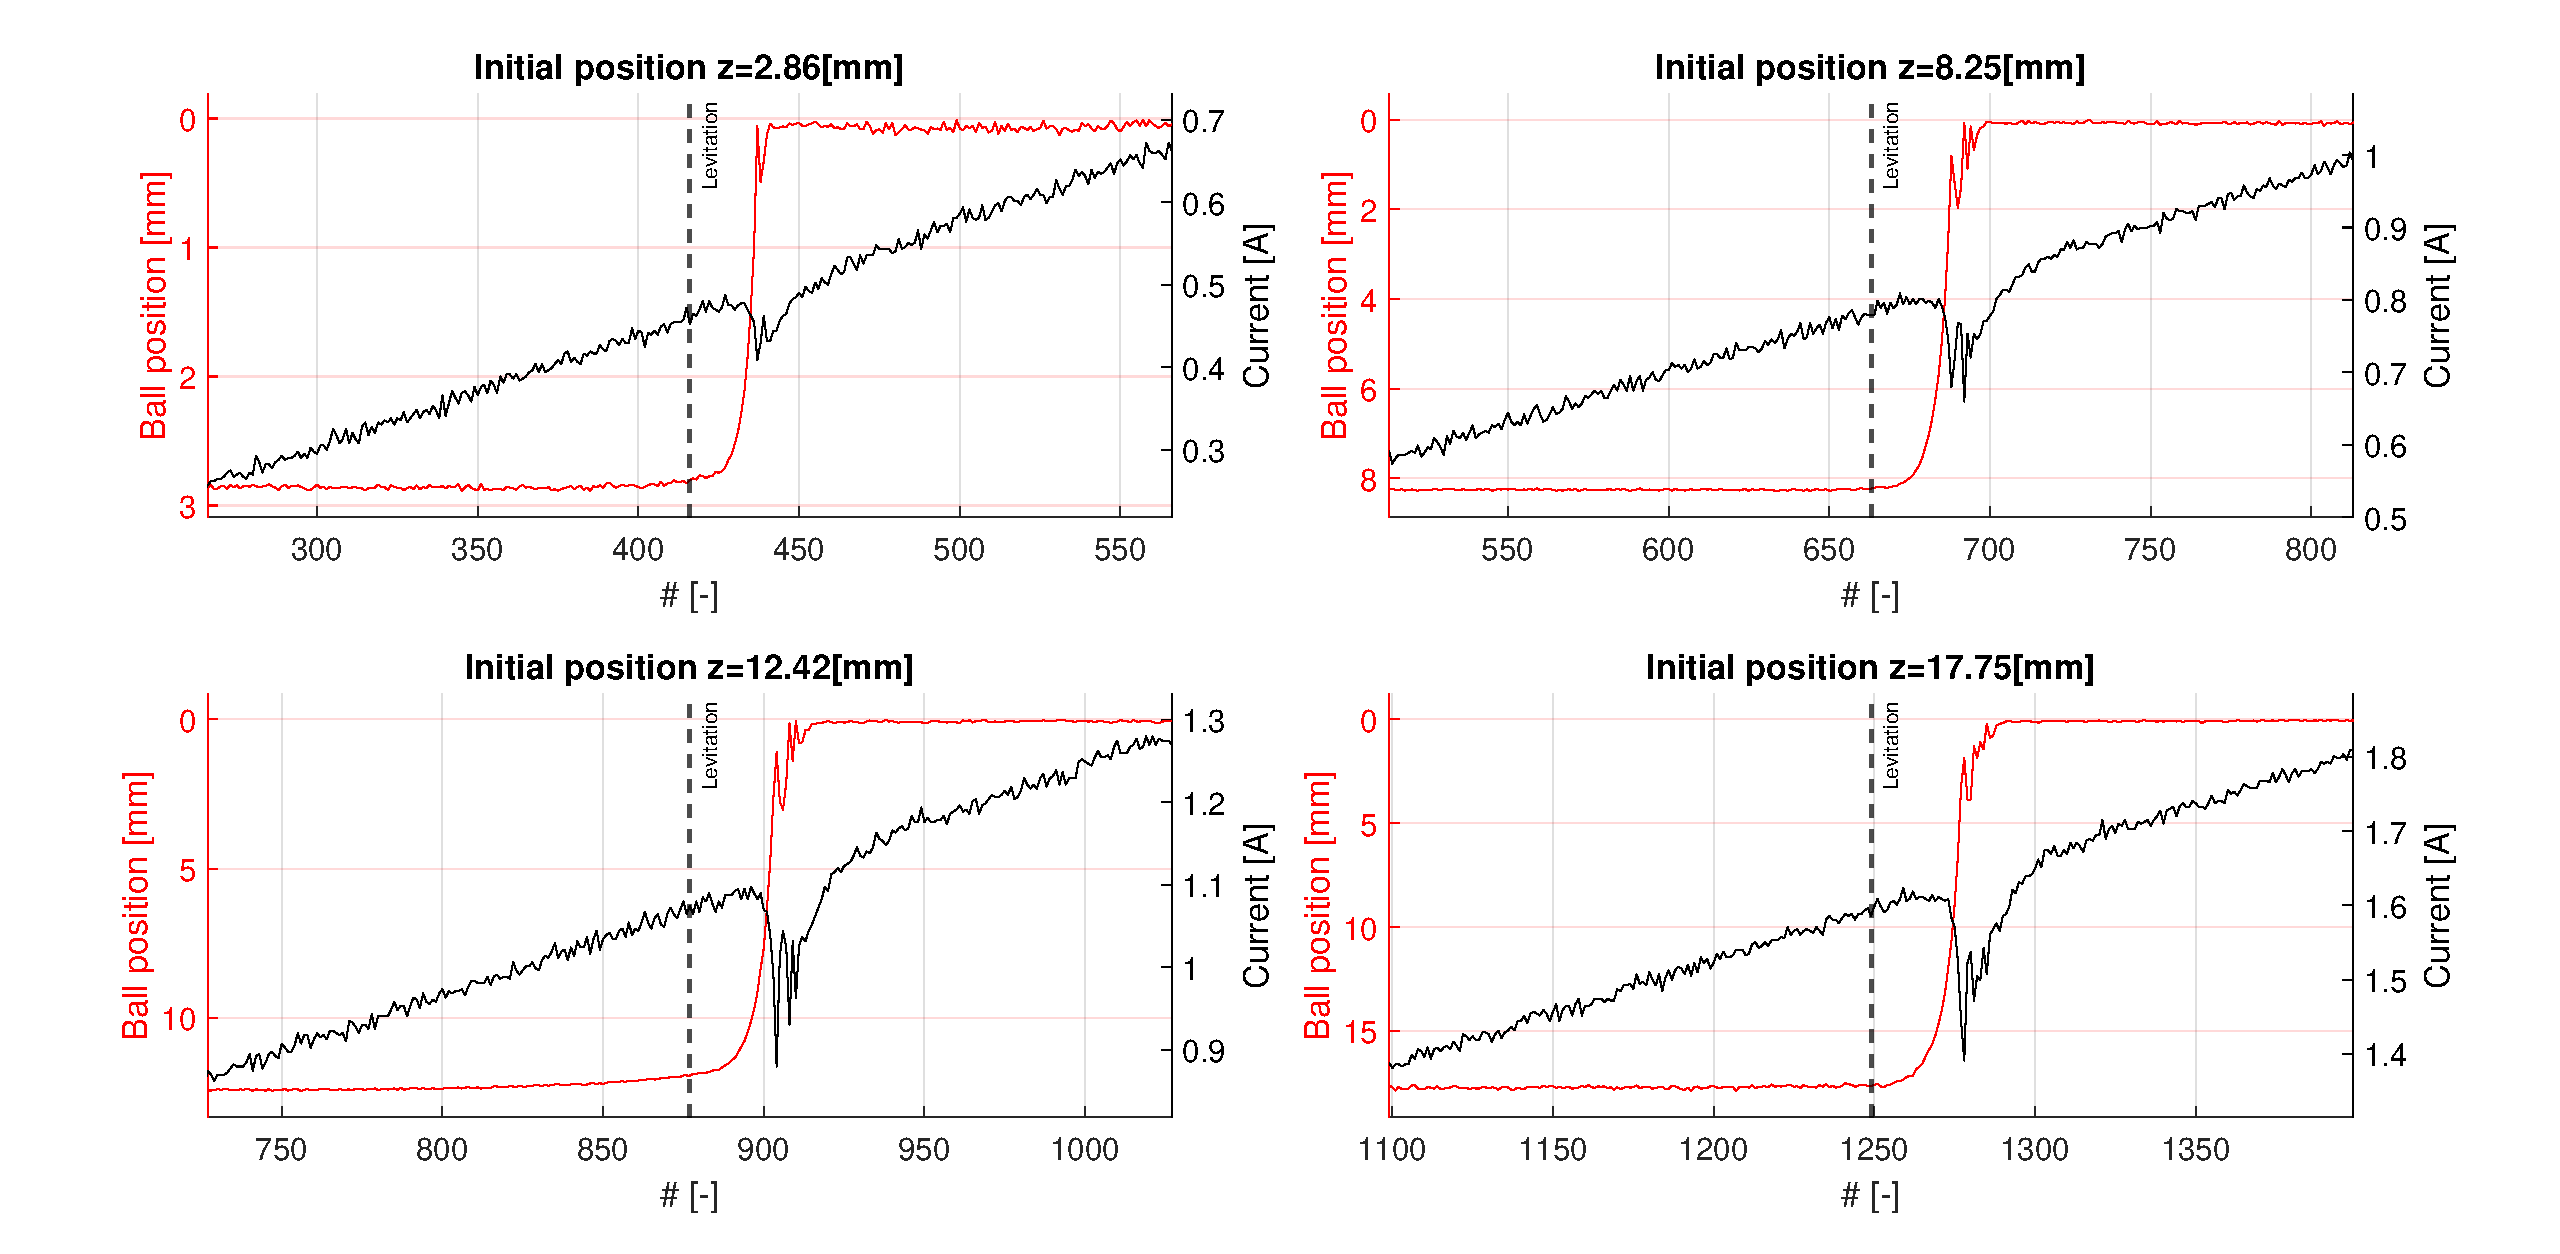
\includegraphics[width=1\textwidth]{img/MATLAB/identification/currents_for_force.pdf}
    \caption{Position of the ball and current in the first coil around the levitation point (marked by vertical black line)}
    \label{fig:levitation_current}
\end{figure}

In Figure \ref{fig:dynamic_inductance_characteristics}, we can observe both the measured data and the fitted ones.
On the right side figure, a complete characterization of the electromagnetic force has been reconstructed based again on the above equations.

\begin{figure}[H]
    \centering
    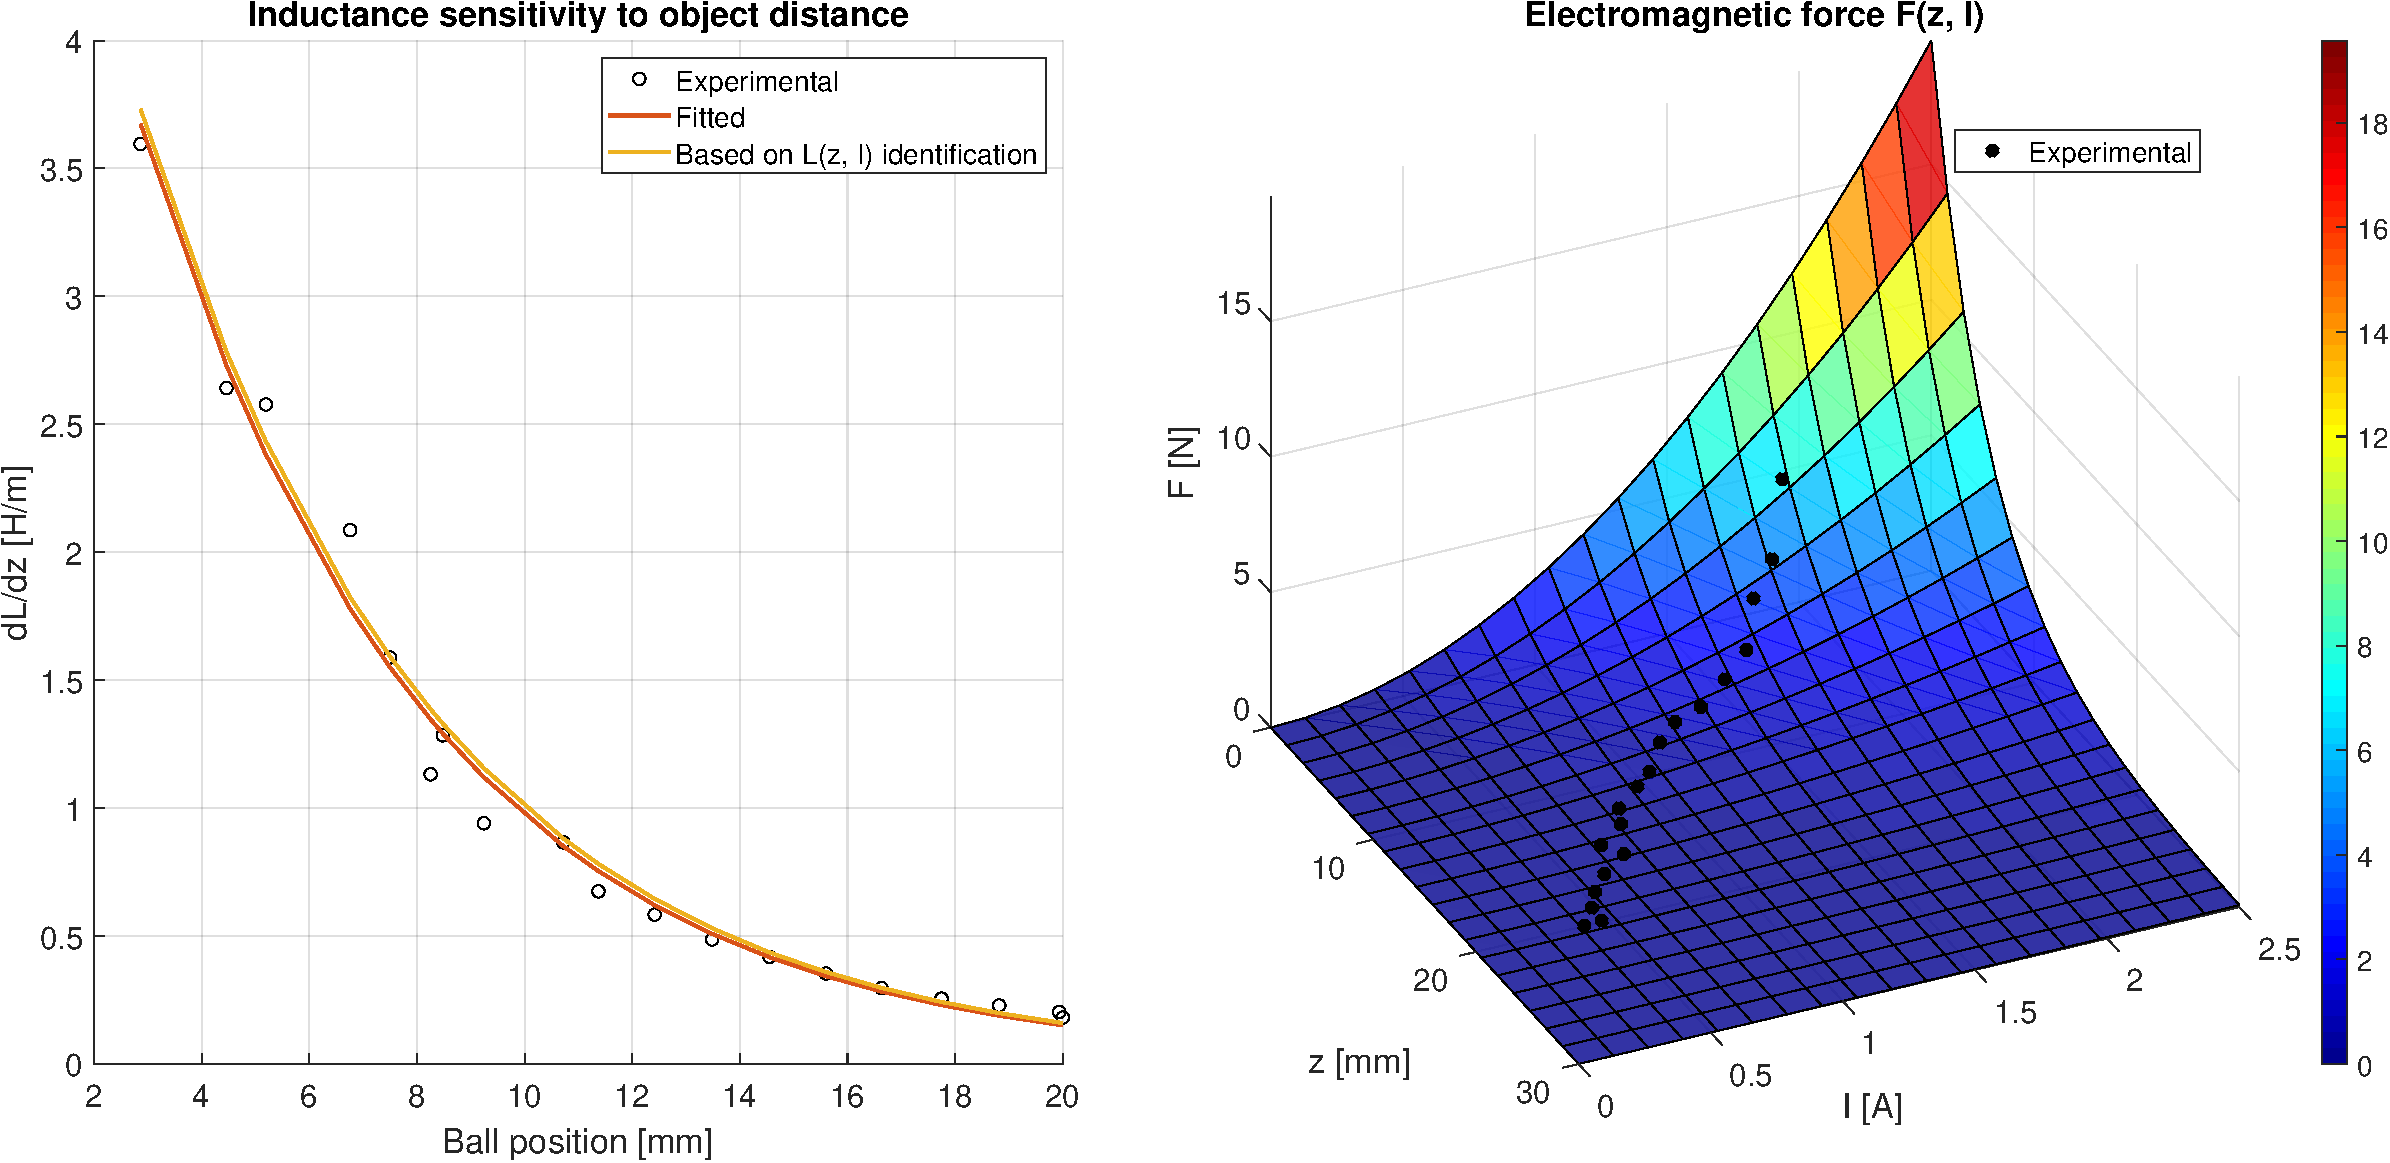
\includegraphics[width=1\textwidth]{img/MATLAB/identification/force.pdf}
    \caption{Dynamic inductance characteristics and electromagnet force}
    \label{fig:dynamic_inductance_characteristics}
\end{figure}

The left-hand side of Figure \ref{fig:dynamic_inductance_characteristics} shows a comparison between the measured data (black circles), their fitting (red line), the sensitivity of the inductance coming from the model (blue line) and the sensitivity of the inductance resulting from the literature parameters (green line).
Notice that the curve coming from the literature parameters has been doubled given the different model used for the electromagnetic force in the literature (see Equation \ref{eq:simplified_equations_of_motion_final}).

Data shows great accuracy in almost the entire range of the ball position, with a slight discrepancy in the lower part of the range.
This discrepancy is probably due to poor measurement quality because of high noise ratio given by the infrared sensor.

The right-hand side of Figure \ref{fig:dynamic_inductance_characteristics} shows the electromagnetic force generated by the first coil as a function of both the ball position and the current circulating in the coil.
One can notice that the force has an exponential behavior with respect to the ball position and a quadratic behavior with respect to the current.